% Executive Summary Dashboard
% 2-page visual spread: hero metrics, system overview, research journey

\cleardoublepage
\thispagestyle{empty}

% ─── PAGE 1: KEY RESULTS ───────────────────────────────────────────

\begin{center}
{\Large\bfseries Executive Summary}\\[4pt]
{\footnotesize\textit{NFL Analytics: A 13-Month Journey from Prediction to Production}}
\end{center}

\vspace{0.8cm}

% Hero metrics row
\begin{center}
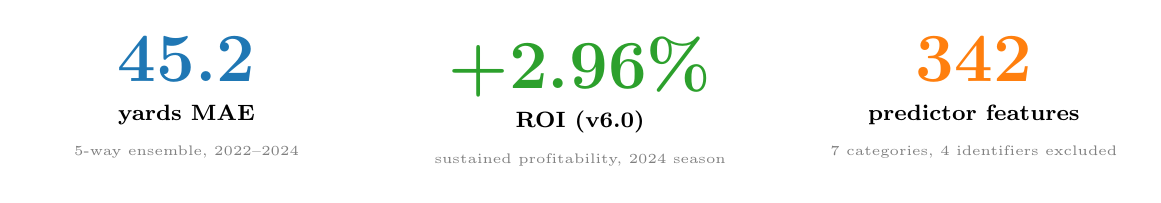
\begin{tikzpicture}
\definecolor{accent}{RGB}{31,119,180}
\definecolor{accentGreen}{RGB}{44,160,44}
\definecolor{accentOrange}{RGB}{255,127,14}

% Metric 1: Prediction accuracy
\node[anchor=north] at (0,0) {
  \begin{minipage}{3.8cm}\centering
    {\fontsize{28}{32}\selectfont\bfseries\color{accent} 45.2}\\[2pt]
    {\footnotesize\bfseries yards MAE}\\[1pt]
    {\tiny\color{black!50} 5-way ensemble, 2022--2024}
  \end{minipage}
};

% Metric 2: Betting ROI
\node[anchor=north] at (5,0) {
  \begin{minipage}{3.8cm}\centering
    {\fontsize{28}{32}\selectfont\bfseries\color{accentGreen} +2.96\%}\\[2pt]
    {\footnotesize\bfseries ROI (v6.0)}\\[1pt]
    {\tiny\color{black!50} sustained profitability, 2024 season}
  \end{minipage}
};

% Metric 3: Feature count
\node[anchor=north] at (10,0) {
  \begin{minipage}{3.8cm}\centering
    {\fontsize{28}{32}\selectfont\bfseries\color{accentOrange} 342}\\[2pt]
    {\footnotesize\bfseries predictor features}\\[1pt]
    {\tiny\color{black!50} 7 categories, 4 identifiers excluded}
  \end{minipage}
};

\end{tikzpicture}
\end{center}

\vspace{0.3cm}

% Second metrics row
\begin{center}
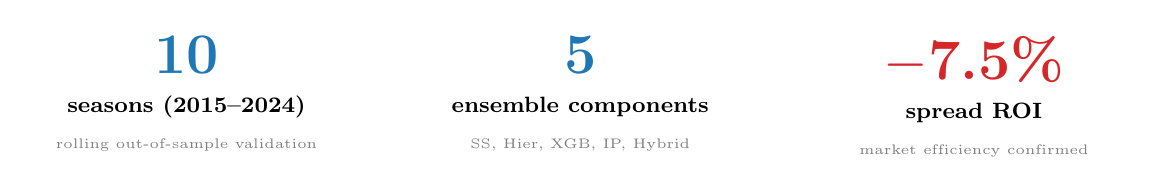
\begin{tikzpicture}
\definecolor{accent}{RGB}{31,119,180}
\definecolor{accentRed}{RGB}{214,39,40}

% Metric 4: Seasons validated
\node[anchor=north] at (0,0) {
  \begin{minipage}{3.8cm}\centering
    {\fontsize{22}{26}\selectfont\bfseries\color{accent} 10}\\[2pt]
    {\footnotesize\bfseries seasons (2015--2024)}\\[1pt]
    {\tiny\color{black!50} rolling out-of-sample validation}
  \end{minipage}
};

% Metric 5: Models in ensemble
\node[anchor=north] at (5,0) {
  \begin{minipage}{3.8cm}\centering
    {\fontsize{22}{26}\selectfont\bfseries\color{accent} 5}\\[2pt]
    {\footnotesize\bfseries ensemble components}\\[1pt]
    {\tiny\color{black!50} SS, Hier, XGB, IP, Hybrid}
  \end{minipage}
};

% Metric 6: Market efficiency finding
\node[anchor=north] at (10,0) {
  \begin{minipage}{3.8cm}\centering
    {\fontsize{22}{26}\selectfont\bfseries\color{accentRed} $-$7.5\%}\\[2pt]
    {\footnotesize\bfseries spread ROI}\\[1pt]
    {\tiny\color{black!50} market efficiency confirmed}
  \end{minipage}
};

\end{tikzpicture}
\end{center}

\vspace{0.6cm}

% Key findings box
\begin{tcolorbox}[
  colback=accentBlue!3,
  colframe=accentBlue!40,
  title={\small\bfseries Core Findings},
  fonttitle=\bfseries\small,
  boxrule=0.5pt,
  left=6pt, right=6pt, top=4pt, bottom=4pt
]
\small
\begin{enumerate}[itemsep=2pt, parsep=0pt, leftmargin=*]
  \item \textbf{Prediction accuracy $\neq$ betting profitability.} The ensemble achieves strong MAE (45.2 yards) but spread betting ROI is $-7.5\%$---the market is efficient for standard bets.
  \item \textbf{Profitability exists in market microstructure.} Edge-based selection, timing, and alternative lines yield $+2.96\%$ ROI through the profit optimization framework.
  \item \textbf{Ensemble diversity $>$ individual model sophistication.} The 5-way ensemble outperforms every component; low error correlations (0.34--0.79) drive the gain.
  \item \textbf{Feature pipeline health $>$ model complexity.} Market microstructure features ($+6.15\%$ MAE impact) matter more than model architecture choices.
  \item \textbf{Honest evaluation prevents self-deception.} Temporal splits, leakage audits, and multi-season validation exposed multiple instances of inflated performance.
\end{enumerate}
\end{tcolorbox}

\vspace{0.5cm}

% Simplified architecture diagram
\begin{center}
{\small\bfseries System Architecture (v6.0)}\\[6pt]
\begin{tikzpicture}[
  node distance=0.8cm,
  box/.style={rectangle, draw=accentBlue!60, fill=accentBlue!8, rounded corners=2pt, font=\tiny, minimum width=2cm, minimum height=0.6cm, align=center},
  arrow/.style={->, thick, accentBlue!60}
]
% Data layer
\node[box, minimum width=3cm] (data) {342 Features\\7 categories};

% Models
\node[box, above right=0.6cm and -1cm of data] (ss) {State-Space v2\\27\%};
\node[box, right=0.3cm of ss] (hier) {Hierarchical v2\\27\%};
\node[box, right=0.3cm of hier] (xgb) {XGBoost v4\\23\%};
\node[box, right=0.3cm of xgb] (ip) {Inform.\ Priors\\13\%};
\node[box, right=0.3cm of ip] (hyb) {Hybrid\\10\%};

% Ensemble
\node[box, above=0.6cm of xgb, minimum width=3cm, fill=accentBlue!15, draw=accentBlue] (ens) {WLS Ensemble\\45.2 MAE};

% Profit
\node[box, above=0.6cm of ens, minimum width=3.5cm, fill=green!8, draw=green!50!black] (profit) {Profit Optimization\\+2.96\% ROI};

% Arrows
\draw[arrow] (data) -- (ss);
\draw[arrow] (data) -- (hier);
\draw[arrow] (data) -- (xgb);
\draw[arrow] (data) -- (ip);
\draw[arrow] (data) -- (hyb);
\draw[arrow] (ss) -- (ens);
\draw[arrow] (hier) -- (ens);
\draw[arrow] (xgb) -- (ens);
\draw[arrow] (ip) -- (ens);
\draw[arrow] (hyb) -- (ens);
\draw[arrow] (ens) -- (profit);

\end{tikzpicture}
\end{center}

% ─── PAGE 2: RESEARCH JOURNEY ──────────────────────────────────────

\clearpage
\thispagestyle{empty}

\begin{center}
{\Large\bfseries Research Journey}\\[4pt]
{\footnotesize\textit{13 months from catastrophic failure to sustained profitability}}
\end{center}

\vspace{0.5cm}

\begin{center}
\begin{tikzpicture}[
  node distance=1.2cm,
  phase/.style={rectangle, draw=#1!60, fill=#1!10, rounded corners=3pt, font=\scriptsize, text width=3.2cm, align=center, minimum height=1.2cm},
  milestone/.style={circle, draw=#1!60, fill=#1!20, font=\tiny\bfseries, inner sep=2pt, minimum size=0.5cm},
  timeline/.style={very thick, accentBlue!40},
  label/.style={font=\tiny, text=black!50, text width=2cm, align=center}
]

\definecolor{fail}{RGB}{214,39,40}
\definecolor{discover}{RGB}{44,160,44}
\definecolor{build}{RGB}{31,119,180}
\definecolor{crisis}{RGB}{255,127,14}

% Timeline backbone (vertical)
\draw[timeline] (0,0) -- (0,-13);

% Phase 1: Initial failure
\node[milestone=fail] at (0,0) {1};
\node[phase=fail, anchor=west] at (0.6,0) {\textbf{Oct 2024}\\v1.0: Single model\\$-3.75\%$ ROI, $-83.5\%$ DD};
\node[label, anchor=east] at (-0.5,0) {Catastrophic\\failure};

% Phase 2: Ensemble discovery
\node[milestone=discover] at (0,-2) {2};
\node[phase=discover, anchor=east] at (-0.6,-2) {\textbf{Nov 2024}\\v2.5: First ensemble\\$+1.50\%$ ROI (breakthrough)};
\node[label, anchor=west] at (0.5,-2.5) {2-way ensemble\\changes everything};

% Phase 3: XGBoost integration
\node[milestone=build] at (0,-4) {3};
\node[phase=build, anchor=west] at (0.6,-4) {\textbf{Nov 2024}\\v3.0: XGBoost added\\$+2.21\%$ ROI, 47.8 MAE};

% BNN dead end (branch)
\draw[dashed, fail!50, thick] (0,-3) -- (-3.5,-4.5);
\node[phase=fail, anchor=east, text width=2.8cm] at (-3.5,-4.5) {\textbf{BNN Dead End}\\84 hours, 6 approaches\\abandoned Nov 9};

% Phase 4: Leakage crisis
\node[milestone=crisis] at (0,-6) {4};
\node[phase=crisis, anchor=east] at (-0.6,-6) {\textbf{Nov 2025}\\Leakage audit\\inflated metrics found};
\node[label, anchor=west] at (0.5,-6.5) {Honest evaluation\\saves integrity};

% Phase 5: v5.0 recovery
\node[milestone=build] at (0,-8) {5};
\node[phase=build, anchor=west] at (0.6,-8) {\textbf{Nov 2025}\\v5.0--5.1: Clean rebuild\\$+2.80\%$ ROI, 44.5 MAE};

% Phase 6: Production
\node[milestone=discover] at (0,-10) {6};
\node[phase=discover, anchor=east] at (-0.6,-10) {\textbf{Dec 2025}\\v6.0: 5-way adaptive\\$+2.96\%$ ROI, 44.25 MAE};

% Props pipeline (branch)
\draw[dashed, crisis!50, thick] (0,-9) -- (3.5,-10.5);
\node[phase=crisis, anchor=west, text width=2.8cm] at (3.5,-10.5) {\textbf{Props Discovery}\\v8.0 Dirichlet weights\\79\% Bayesian dominance};

% Phase 7: Current state
\node[milestone=discover] at (0,-12) {7};
\node[phase=discover, anchor=west] at (0.6,-12) {\textbf{2025 Holdout}\\74.9\% spread accuracy\\true OOS validation};

% Improvement arrow
\draw[->, very thick, discover!60] (-4.5,-12.5) -- (-4.5,0.5);
\node[font=\tiny\bfseries, text=discover!80!black, rotate=90, anchor=south] at (-4.8,-6) {MAE: 62.3 $\to$ 44.25 ($-$29\%) \quad ROI: $-$3.75\% $\to$ $+$2.96\%};

\end{tikzpicture}
\end{center}

\vspace{0.3cm}

% Key lesson callout
\begin{tcolorbox}[
  colback=black!2,
  colframe=black!30,
  boxrule=0.4pt,
  left=6pt, right=6pt, top=3pt, bottom=3pt
]
\small\itshape
\textbf{The central lesson:} The path to a working system was not a straight line. It required abandoning 84 hours of BNN research, surviving a data leakage crisis, and learning that prediction accuracy alone does not guarantee profitability. The final system works not because any single component is exceptional, but because five imperfect models, combined honestly, cover each other's weaknesses.
\end{tcolorbox}
